\subsubsection{Aggiornamento Risorse Rimaste}
\label{sec:AggiornamentoRisorse_Sprint11}
Al termine dello \textbf{\glossario{Sprint} 11} rimangono le seguenti ore per ruolo: \hyperref[tab:sprint11_ore_rimanenti]{In tabella \ref{tab:sprint11_ore_rimanenti}} vengono mostrate le ore rimanenti per ruolo al termine dello \textit{\glossario{Sprint} 11}.

\begin{table}[H]
    \centering
    \begin{tabular}{| l | l | l|}
    \hline
    \textbf{Ruolo} & \textbf{Ore preventivate fino al PB} & \textbf{Ore rimanenti fino al PB}\\
    \hline
        Responsabile & 23.75 & 17.25 \\
    \hline
        Amministratore & 22 & 5.5 \\
    \hline
        Programmatore & 90 & 90 \\
    \hline
        Analista & 0 & 0 \\
    \hline
        Verificatore & 109.75 & 72.25 \\
    \hline
        Progettista & 105 & 69.15 \\
    \hline
    \end{tabular}
    \caption{Ore rimanenti per ruolo.}
    \label{tab:sprint11_ore_rimanenti} 
\end{table}

\begin{figure}[H]
    \centering
    \resizebox{\textwidth}{!}{
    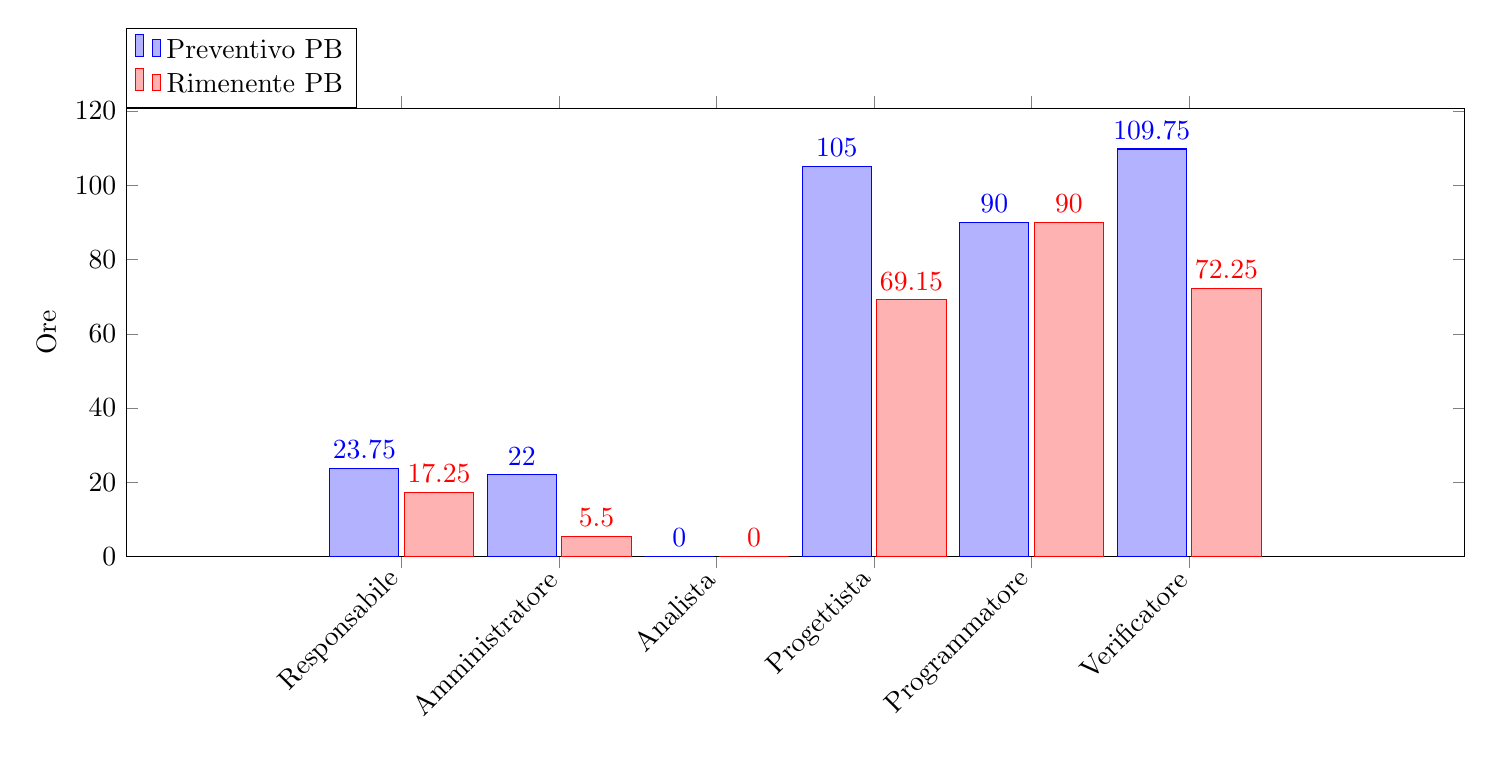
\begin{tikzpicture}
        \begin{axis}[
            ybar,
            symbolic x coords={Responsabile, Amministratore, Analista, Progettista, Programmatore, Verificatore},
            xtick=data,
            nodes near coords,
            ymin=0,
            ylabel={Ore},
            enlarge x limits=0.35,
            bar width=25pt,
            xticklabel style={rotate=45, anchor=east},
            x=2cm,
            legend style={at={(0,1)}, anchor=south west, legend columns=1}
        ]

            \addplot coordinates {(Amministratore,22) (Responsabile,23.75) (Analista,0) (Progettista, 105) (Programmatore, 90) (Verificatore, 109.75)};
            \addplot coordinates {(Amministratore,5.5) (Responsabile,17.25) (Analista, 0) (Progettista, 69.15) (Programmatore, 90) (Verificatore, 72.25)};

            \legend{Preventivo PB, Rimenente PB}

        \end{axis}
    \end{tikzpicture}}
    \caption{Grafico di confronto tra le risorse preventivate e rimanenti.}
    \label{fig:sprint11_risorse_rimanenti}
\end{figure}